\documentclass{article}

% The official Overleaf template loads this package from the template project:
% https://www.overleaf.com/latex/templates/template-for-iclr-2025-conference-submission/gqzkdyycxtvt
\usepackage{iclr2025_conference,times}

\usepackage{hyperref}
\usepackage{url}
\usepackage{booktabs}
\usepackage{amsmath}
\usepackage{amssymb}
\usepackage{graphicx}
\usepackage{tikz}
\usetikzlibrary{arrows.meta,positioning,fit}

\title{Progress Report: Channel-Gated Partial Convolution for FasterNet}

\author{
Erkani Mert Tosun \\
Department of Computer Engineering \\
Hacettepe University \\
\texttt{N25123091}
}

% Uncomment for final/camera-ready formatting if requested by the instructor.
\iclrfinalcopy

\begin{document}

\maketitle

\begin{abstract}
This progress report studies a lightweight extension of FasterNet, a latency-oriented convolutional network built around partial convolution (PConv). FasterNet shows that low FLOPs do not necessarily imply low latency, and therefore applies spatial convolution only to a subset of feature channels to improve effective hardware utilisation. We propose a Channel Gate Module (CGM) inserted immediately after PConv. CGM operates only on the spatially processed channel subset and adaptively rescales these channels before pointwise mixing. We implemented FasterNet-T0/T1 and several CGM placements in PyTorch, then evaluated them on CIFAR-100 with accuracy, parameter, FLOP, latency, and gate-statistics measurements. Preliminary results suggest that selective early-stage CGM gives a small accuracy gain, while gating too many stages increases latency without a comparable benefit.
\end{abstract}

\section{Problem Definition}

Modern vision networks must balance accuracy with inference efficiency. This is especially important for edge devices, robotics, and real-time perception, where memory traffic and latency can be as important as top-1 accuracy. A common efficient-CNN strategy is to reduce FLOPs, for example by replacing standard convolutions with depthwise convolutions. However, FasterNet argues that FLOPs alone are an incomplete speed proxy: an operator with few arithmetic operations can still be slow if it causes inefficient memory access or poor hardware utilisation \citep{chen2023fasternet}.

Within this framing, the project investigates the following research question:
\begin{quote}
\emph{Can a lightweight, channel-attention style module operating only on the PConv-processed channel subset improve the predictive accuracy of FasterNet without eliminating its latency advantage?}
\end{quote}
In the original FasterNet block, PConv applies a $3 \times 3$ convolution to only a fraction of the channels and leaves the remaining channels unchanged; a pointwise MLP then mixes information across all channels. This is efficient, but all PConv-processed channels are forwarded uniformly. Our extension tests whether a small input-adaptive gate can prioritise useful PConv channels before the following pointwise convolution.

The main challenges are: \emph{(i)} the added module must remain lightweight enough to preserve FasterNet's motivation; \emph{(ii)} latency must be measured directly rather than inferred only from FLOPs; \emph{(iii)} full ImageNet training is infeasible for this course project, so the experiments must use smaller benchmarks while remaining meaningful; and \emph{(iv)} because the proposed gate is input-dependent, we should inspect whether it learns non-trivial channel preferences rather than acting as a constant scale.

\section{Related Work}

Efficient CNN design has often focused on reducing arithmetic cost. MobileNetV1 introduced depthwise separable convolution \citep{howard2017mobilenets}, MobileNetV2 added inverted residual blocks and linear bottlenecks \citep{sandler2018mobilenetv2}, and ShuffleNet/ShuffleNetV2 used grouped pointwise convolutions, channel shuffle, and practical low-latency design rules \citep{zhang2018shufflenet,ma2018shufflenetv2}. EfficientNet later proposed compound scaling under a fixed resource budget \citep{tan2019efficientnet}. These models show that compact architectures matter, but ShuffleNetV2 and FasterNet also emphasise that memory access, operator fragmentation, and hardware utilisation can dominate actual latency.

Modern convolutional backbones remain competitive when carefully designed. ConvNeXt revisited ConvNet design with transformer-era training and architectural choices \citep{liu2022convnext}. FasterNet continues this CNN line but focuses more directly on latency by using PConv: only a subset of channels receives spatial convolution, while pointwise layers handle cross-channel mixing \citep{chen2023fasternet}.

Our extension is inspired by channel attention. Squeeze-and-Excitation Networks globally pool feature maps and use a small bottleneck MLP with a sigmoid gate to rescale channels \citep{hu2018senet}; CBAM adds spatial attention as well \citep{woo2018cbam}; and ECA-Net replaces the SE bottleneck with lightweight 1D channel convolution \citep{wang2020eca}. Unlike a generic attention insertion, our CGM is restricted to the PConv-processed subset, so the extension remains aligned with FasterNet's partial-channel computation principle.

\section{Method}

\paragraph{Design rationale.} We designed CGM by following two constraints from FasterNet. First, the extension should not turn the block back into a heavy attention module, so the gate is restricted to the PConv-processed channels instead of all channels. Second, because latency is sensitive to memory movement and small element-wise operators, we treat placement as part of the design: gating every block may not be the best choice even if the parameter and FLOP overhead is small. This led us to evaluate selective early-stage and per-stage placements rather than only a single ``CGM everywhere'' model.

\subsection{Base method: FasterNet and partial convolution}

FasterNet \citep{chen2023fasternet} is built around the observation that a network should be evaluated not only by FLOPs but also by its achieved computational throughput. A standard convolution performs spatial mixing for every input and every output channel, which is accurate but expensive. Depthwise convolution reduces FLOPs by applying spatial filtering independently per channel, but in many architectures this requires increasing width to recover accuracy; wider layers in turn increase memory traffic, and the resulting model can have low actual FLOPS.

PConv offers a different trade-off. Given an input tensor $X \in \mathbb{R}^{B \times C \times H \times W}$, the channels are split into two parts:
\begin{equation}
X = [X_p, X_u],
\end{equation}
where $X_p$ contains $C_p = C / n$ channels and $X_u$ contains the remaining untouched channels. PConv applies a $3 \times 3$ convolution only to $X_p$:
\begin{equation}
\hat{X}_p = \mathrm{Conv}_{3 \times 3}(X_p),
\end{equation}
and concatenates the result with $X_u$:
\begin{equation}
\hat{X} = [\hat{X}_p, X_u].
\end{equation}
The following pointwise convolutional MLP mixes information across channels. In the official FasterNet implementation, the main block applies PConv as spatial mixing, then a two-layer pointwise MLP with normalisation and activation, and finally adds the residual shortcut. Figure~\ref{fig:base_block} summarises this block structure.

\begin{figure}[t]
\centering
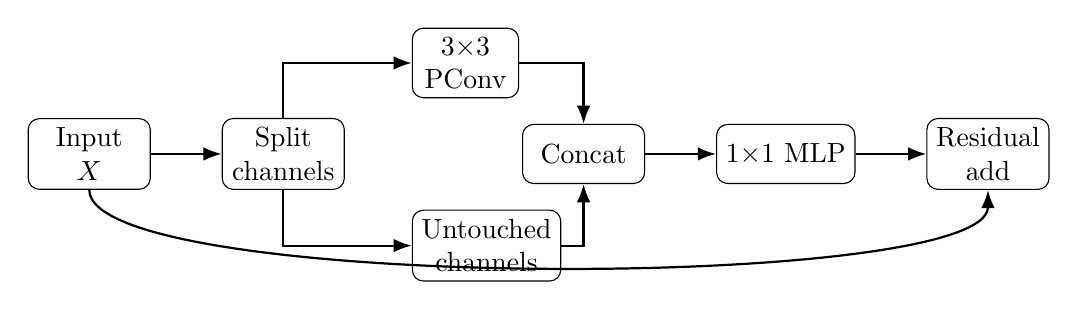
\begin{tikzpicture}[
    node distance=0.9cm,
    block/.style={draw, rounded corners, align=center, minimum height=0.75cm, minimum width=1.55cm},
    smallblock/.style={draw, rounded corners, align=center, minimum height=0.65cm, minimum width=1.35cm},
    arrow/.style={-Latex, thick}
]
\node[block] (x) {Input\\$X$};
\node[block, right=of x] (split) {Split\\channels};
\node[smallblock, above right=0.25cm and 0.85cm of split] (pconv) {$3{\times}3$\\PConv};
\node[smallblock, below right=0.25cm and 0.85cm of split] (id) {Untouched\\channels};
\node[block, right=2.25cm of split] (concat) {Concat};
\node[block, right=of concat] (mlp) {$1{\times}1$ MLP};
\node[block, right=of mlp] (add) {Residual\\add};
\draw[arrow] (x) -- (split);
\draw[arrow] (split) |- (pconv);
\draw[arrow] (split) |- (id);
\draw[arrow] (pconv) -| (concat);
\draw[arrow] (id) -| (concat);
\draw[arrow] (concat) -- (mlp);
\draw[arrow] (mlp) -- (add);
\draw[arrow] (x.south) .. controls +(0,-1.3) and +(0,-1.3) .. (add.south);
\end{tikzpicture}
\caption{Simplified FasterNet block. PConv performs spatial mixing on a subset of channels, while the pointwise MLP performs cross-channel mixing.}
\label{fig:base_block}
\end{figure}

\subsection{Proposed extension: Channel Gate Module}

CGM is inserted immediately after PConv. Instead of recalibrating all $C$ channels, the gate is applied only to the $C_p$ channels that were spatially processed. Let $\hat{X}_p \in \mathbb{R}^{B \times C_p \times H \times W}$ be the PConv output. CGM first computes a global average pooled descriptor:
\begin{equation}
z_c = \frac{1}{HW}\sum_{i=1}^{H}\sum_{j=1}^{W} \hat{X}_{p,c,i,j}.
\end{equation}
The descriptor is passed through a bottleneck MLP, producing per-channel logits $a$, and then a sigmoid:
\begin{equation}
a = W_2 \delta(W_1 z), \qquad g = \sigma(a),
\end{equation}
where $\delta$ is ReLU, $\sigma$ is sigmoid, $W_1 \in \mathbb{R}^{C_p/r \times C_p}$, $W_2 \in \mathbb{R}^{C_p \times C_p/r}$, and $r$ is a reduction ratio (default $r{=}4$). The base \emph{sigmoid} gate scales each channel by $g_c \in [0,1]$:
\begin{equation}
\tilde{X}_{p,c,:,:} = g_c \cdot \hat{X}_{p,c,:,:}.
\end{equation}
The gated tensor $\tilde{X}_p$ is concatenated with the untouched channels and forwarded to the original pointwise MLP, so the FasterNet block topology and its memory access pattern on the untouched channels are not modified.

\paragraph{Implemented variants.} The main preliminary experiments use SE-style CGM with global average pooling, sigmoid scaling, and $r{=}4$. In the codebase we also implemented two close variants: an ECA-style gate \citep{wang2020eca}, which replaces the bottleneck MLP with lightweight 1D channel convolution, and an identity-biased initialisation, where the final gate layer starts near $\sigma(b)\!\approx\!1$ instead of near the sigmoid midpoint. These two variants are not part of the headline tables in this progress report. For placement, we compare \emph{none}, \emph{all}, \emph{early} (stages 1--2), \emph{late} (stages 3--4), and selected per-stage settings (\emph{s1--s4}). This lets us test whether the benefit comes from channel gating in general or from a specific depth. Figure~\ref{fig:cgm} shows where the proposed gate is inserted.

\begin{figure}[t]
\centering
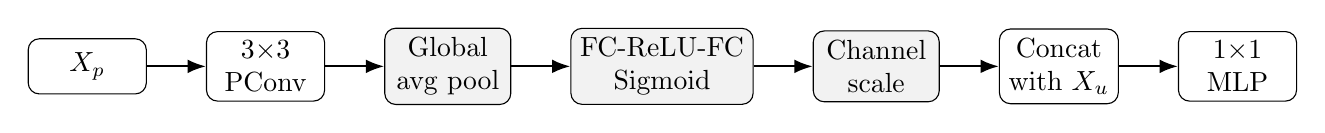
\begin{tikzpicture}[
    node distance=0.75cm,
    block/.style={draw, rounded corners, align=center, minimum height=0.7cm, minimum width=1.5cm},
    gate/.style={draw, rounded corners, align=center, minimum height=0.7cm, minimum width=1.6cm, fill=gray!10},
    arrow/.style={-Latex, thick}
]
\node[block] (xp) {$X_p$};
\node[block, right=of xp] (pconv) {$3{\times}3$\\PConv};
\node[gate, right=of pconv] (gap) {Global\\avg pool};
\node[gate, right=of gap] (fc) {FC-ReLU-FC\\Sigmoid};
\node[gate, right=of fc] (scale) {Channel\\scale};
\node[block, right=of scale] (cat) {Concat\\with $X_u$};
\node[block, right=of cat] (pw) {$1{\times}1$\\MLP};
\draw[arrow] (xp) -- (pconv);
\draw[arrow] (pconv) -- (gap);
\draw[arrow] (gap) -- (fc);
\draw[arrow] (fc) -- (scale);
\draw[arrow] (scale) -- (cat);
\draw[arrow] (cat) -- (pw);
\end{tikzpicture}
\caption{Channel Gate Module. The gate is restricted to the PConv-processed channel subset, which limits overhead while still enabling input-adaptive recalibration before the pointwise MLP.}
\label{fig:cgm}
\end{figure}

\section{Experimental Settings and Preliminary Results}

\subsection{Datasets and evaluation metrics}

The original FasterNet paper reports ImageNet-1K classification, which is computationally infeasible at the course-project scale. We therefore use CIFAR-100 \citep{krizhevsky2009cifar} as the benchmark for this progress report (60{,}000 images, 100 classes, native $32{\times}32$, 50k train / 10k val). We report top-1 validation accuracy together with three efficiency metrics: parameter count, FLOPs (computed via \texttt{fvcore} on a single $1{\times}3{\times}H{\times}W$ input), and measured GPU latency.

\subsection{Implementation and training protocol}

We re-implemented FasterNet-T0 ($\mathrm{embed\_dim}{=}40$, depths $(1,2,8,2)$) and FasterNet-T1 ($\mathrm{embed\_dim}{=}64$, depths $(1,2,8,2)$, $\mathrm{drop\_path}{=}0.02$) in PyTorch, faithful to the official block structure but free of the PyTorch-Lightning / timm dependency stack so that training runs cleanly on Colab and Kaggle GPUs. Datasets are loaded through Hugging Face \texttt{datasets}. For CIFAR-100 we keep the native $32{\times}32$ input and use patch size 2 in both patch-embed and patch-merging layers. All variants are trained with AdamW, cosine learning rate schedule, and batch size 128, for 20 or 40 epochs as noted in each table. The headline placement comparison on T0 is averaged over two random seeds; downstream ablations that drill into the headline result use a single training run to keep the GPU budget within course-project limits. To isolate the effect of CGM, all compared variants share the same training recipe; this also means our training protocol is intentionally simple (no MixUp/CutMix/EMA) so that the gate's effect is not confounded by stronger regularisation. Latency is measured on a single GPU at batch size 1, with 100 warm-up forward passes followed by 200 timed passes; we report the mean across the timed window.

\paragraph{Experimental flow.} The results below should be read as preliminary evidence rather than a final benchmark. We first ran a 20-epoch placement sweep on FasterNet-T0 (\emph{none / early / all / late}) to identify a promising direction. We then used per-stage ablations (\emph{s1--s4}) to understand where the gain comes from, and ran smaller checks on the gate reduction ratio and pooling choice. Finally, we tested whether the same trend appears on the wider FasterNet-T1 with a 40-epoch schedule. Gate statistics are collected on the headline early-stage configurations.

\subsection{Main CIFAR-100 result: placement comparison}

Table~\ref{tab:t0-main} reports the main placement comparison on FasterNet-T0, averaged across seeds 42 and 7 for 20 epochs. CGM-Early gives the best validation accuracy among all four placements ($+0.82$ over the baseline), while CGM-All and CGM-Late add markedly more latency for no clear accuracy benefit. The accuracy gap between CGM-Early and CGM-All is small but the latency gap is large, which indicates that the gain comes from gating early-stage features and not from gating everywhere. We therefore treat CGM-Early as our main candidate configuration in the rest of the experiments and use the per-stage ablation below to identify which early-stage block is responsible for the gain.

\begin{table}[t]
\caption{FasterNet-T0 on CIFAR-100, 20 epochs, 2-seed mean (seeds 42 and 7). Latency is the mean GPU time per image at batch size 1.}
\label{tab:t0-main}
\centering
\small
\begin{tabular}{lrrrrrr}
\toprule
Variant & Seed 42 & Seed 7 & Mean Acc & Params & FLOPs & Latency \\
\midrule
CGM-none  & 50.52 & 50.21 & 50.37 & 2{,}751{,}160 & 27.626\,M & 1.009\,ms \\
CGM-all   & 50.94 & 50.47 & 50.71 & 2{,}765{,}062 & 27.650\,M & 1.674\,ms \\
CGM-early & 51.03 & 51.35 & \textbf{51.19} & 2{,}751{,}662 & 27.632\,M & 1.177\,ms \\
CGM-late  & 50.50 & 50.37 & 50.44 & 2{,}764{,}560 & 27.645\,M & 1.521\,ms \\
\bottomrule
\end{tabular}
\end{table}

\subsection{Per-stage ablation}

Applying CGM to one stage at a time (Table~\ref{tab:t0-stage}) shows that the early-stage gain is mainly driven by stage 2: \emph{s2} reaches 50.89 against 50.52 for the baseline. The single-stage \emph{s3} run produced the highest single-run accuracy (51.39), but a confirmation run reached only 50.29, so we treat \emph{s3} as unstable and expensive rather than as the main result. This supports using \emph{early} as the safer preliminary placement.

\begin{table}[t]
\caption{Per-stage CGM ablation on FasterNet-T0, CIFAR-100, 20 epochs.}
\label{tab:t0-stage}
\centering
\small
\begin{tabular}{lrrrr}
\toprule
Variant & Val Acc & Params & FLOPs & Latency \\
\midrule
none & 50.52 & 2{,}751{,}160 & 27.626\,M & 1.009\,ms \\
s1   & 50.52 & 2{,}751{,}212 & 27.629\,M & 1.084\,ms \\
s2   & 50.89 & 2{,}751{,}610 & 27.629\,M & 1.150\,ms \\
s3   & 51.39 & 2{,}757{,}960 & 27.638\,M & 1.452\,ms \\
s4   & 50.81 & 2{,}757{,}760 & 27.633\,M & 1.144\,ms \\
\bottomrule
\end{tabular}
\end{table}

\paragraph{Reduction ratio and pooling checks.} We also tested whether the default CGM bottleneck ratio and pooling descriptor should be changed. The reduction ratio $r$ controls the hidden width of the gate MLP: $r{=}2$ gives a wider gate, while $r{=}8$ gives a narrower one. On T0 with early CGM, $r{=}2$, $r{=}4$, and $r{=}8$ reached 50.64, 51.03, and 50.39 validation accuracy, respectively; on T1 at 40 epochs they reached 57.06, 57.37, and 56.84. Thus, the default $r{=}4$ remained the best accuracy/overhead choice. We also tried replacing GAP with a GAP+GMP descriptor. This did not improve the early configuration (50.90 on seed 42), and although one selective placement gave a high single-seed result, it dropped on a second seed. For this reason, the headline experiments keep the simpler GAP descriptor.

\subsection{Scaling to FasterNet-T1}

Because T0 is the smallest variant, we ran a 40-epoch protocol on FasterNet-T1 to test whether the early-stage CGM benefit transfers to a larger model and a longer schedule (Table~\ref{tab:t1}; all CGM rows in this table use the base sigmoid mode). At 40 epochs the baseline reaches 56.71 and the \emph{early} variant reaches 57.37 ($+0.66$). Stage-wise gating shows the same trend as on T0: the gain is concentrated in early stages, with \emph{s1} the best accuracy/latency trade-off ($+0.51$ accuracy at only $+0.064$\,ms latency), while late-stage gating (\emph{s3, s4}) produces smaller gains at higher latency cost. We additionally ran a 20-epoch T1 sweep that did \emph{not} show a CGM benefit; we read this together with the 40-epoch result as evidence that CGM's effect on T1 is sensitive to training length.

\begin{table}[t]
\caption{FasterNet-T1 on CIFAR-100, 40 epochs. ``Gain'' is val-acc difference vs.\ the baseline.}
\label{tab:t1}
\centering
\small
\begin{tabular}{lrrrrr}
\toprule
Variant & Val Acc & Gain & Params & FLOPs & Latency \\
\midrule
none                    & 56.71 & --    & 6{,}440{,}164 & 69.807\,M & 1.056\,ms \\
early & \textbf{57.37} & $+0.66$ & 6{,}441{,}416 & 69.816\,M & 1.244\,ms \\
s1    & 57.22 & $+0.51$ & 6{,}440{,}312 & 69.811\,M & 1.120\,ms \\
s2    & 57.20 & $+0.49$ & 6{,}441{,}268 & 69.812\,M & 1.191\,ms \\
s3    & 56.95 & $+0.24$ & 6{,}457{,}188 & 69.832\,M & 1.517\,ms \\
s4    & 56.84 & $+0.13$ & 6{,}456{,}868 & 69.825\,M & 1.181\,ms \\
\bottomrule
\end{tabular}
\end{table}

\subsection{Discussion of preliminary results}

Three observations carry the preliminary story. \emph{First}, selective early-stage CGM gives a small accuracy improvement on CIFAR-100: $+0.82$ averaged over two seeds on T0 at 20 epochs and $+0.66$ on T1 at 40 epochs, with the per-stage ablation pointing to early stages as the useful locations. \emph{Second}, the latency cost is small in absolute terms but is \emph{not} zero, and is much larger than the FLOP cost would suggest: CGM-Early increases FLOPs by less than $0.1\%$ but increases measured GPU latency by roughly $17\%$ on T0, while CGM-All raises latency by roughly $65\%$ for almost identical FLOPs. This reinforces FasterNet's central claim that FLOP count alone is an inadequate proxy for inference speed. \emph{Third}, the gain is preliminary and training-regime dependent: on a longer 40-epoch T0 run, the baseline reaches 55.51 and the early CGM variant reaches 55.68, so the gap shrinks to $+0.17$. Gate statistics also show that sigmoid gates stay near $0.5$ on average but exhibit larger per-channel spread in deeper early blocks and in T1, suggesting non-constant but still preliminary channel behaviour.

\subsection{Future work toward the final report}\label{sec:future}

For the final report, we will first strengthen the training recipe with augmentations such as TrivialAugment, MixUp, and EMA, applying the same recipe to both baseline and CGM models. Beyond the current ablations, we plan to test two FasterNet-specific extensions: a separate lightweight gate for the untouched bypass channels, and sparse stage-3 gating where only selected blocks in the expensive third stage receive CGM. These variants directly target the accuracy-latency trade-off observed in the preliminary results. We will also evaluate centred/residual scaling, extend the gate analysis with correct/incorrect validation examples, and test CGM in a fine-tuning setting using official ImageNet-pretrained FasterNet checkpoints, especially for higher-resolution benchmarks such as Tiny-ImageNet where scratch training may require stronger regularisation.

{\small
\bibliography{references}
\bibliographystyle{iclr2025_conference}
}

\end{document}
